\documentclass{report}

\usepackage[T1]{fontenc}
\usepackage[utf8]{inputenc}
\usepackage[brazilian]{babel}
\usepackage{graphicx}
\usepackage[export]{adjustbox}[2011/08/13]
\usepackage{float}
\usepackage[pdftex]{hyperref}
\usepackage{epstopdf}
\usepackage{etoolbox}
\usepackage{amsmath}
\usepackage{amsfonts}
\usepackage{amssymb}
\usepackage{caption}
\usepackage{subcaption}
\usepackage{setspace}
\usepackage{tikz}
\usepackage{listings}
\usepackage{xcolor} 

\bibliographystyle{eric}
\patchcmd{\thebibliography}{\section*}{\section}{}{}


\newcommand{\R}{\ensuremath{\mathbb{R}}}
\newcommand{\Prob}{\ensuremath{\mathbb{P}}}
\newcommand{\K}{\ensuremath{\mathbb{K}}}
\newcommand{\U}{\ensuremath{\mathbb{U}}}
\newcommand{\N}{\ensuremath{\mathbb{N}}}
\newcommand{\Lg}{\ensuremath{\mathbb{L}}}
\newcommand{\T}{\ensuremath{\rm Tr}}
\newcommand{\sg}{{\sigma(x_k)}}

\newcommand{\G}{\ensuremath{\mathcal{G}}}
\newcommand{\F}{\ensuremath{\mathcal{F}}}
\newcommand{\C}{\ensuremath{\mathcal{C}}}
\newcommand{\E}{\ensuremath{\mathcal{E}}}
\newcommand{\Hn}{\ensuremath{\mathcal{H}}}
\newcommand{\Hoo}{\ensuremath{\mathcal{H}_\infty}}
\newcommand{\Hop}{\ensuremath{\mathcal{H}_{op}}}
% --------------------------------------------------
\newtheorem{theo}{Teorema}
\newtheorem{exa}{Exemplo}
\newtheorem{lemm}{Lema}
\newtheorem{coro}{Corolário}
\newtheorem{defn}{Definição}[section]

\begin{document}

\begin{titlepage}
\begin{center}

\newcommand{\HRule}{\rule{\linewidth}{0.5mm}}
% Upper part of the page. The '~' is needed because \\
% only works if a paragraph has started.

\includegraphics[width=0.15\textwidth]{logoUnicamp}~\\[1cm]

\textsc{\LARGE Universidade Estadual de Campinas}\\[1.5cm]

\textsc{\Large Faculdade de Engenharia Mecânica}\\[0.5cm]

% Title
\HRule \\[0.4cm]
{ \huge \bfseries ES664 - Laboratório de Eletrônica para Automação Industrial\\ \vspace{1cm} Relatório - Experimento 4\\
\Large{Acionamento de motor DC} \\[0.4cm] }

\HRule \\[1.5cm]

% Author and supervisor
\begin{minipage}{0.6\textwidth}
\begin{flushleft} \large
\emph{Nome:}\\
Daniel Dello Russo Oliveira\\Marcelli Tiemi Kian
\end{flushleft}
\end{minipage}
\begin{minipage}{0.2\textwidth}
\begin{flushright} \large
\emph{RA}\\ 101918\\117892
\end{flushright}
\end{minipage}

\vfill

% Bottom of the page
{\large \today}

\end{center}
\end{titlepage}


\onehalfspacing
\section{Objetivos}
	Essa relatório tem como objetivo o estudo de retificadores controlados. Analisaremos o efeito do ângulo de disparo e de cargas indutivas na saída de um retificador monofásico controlado.
	 
\section{Carga R}
Implementamos o retificador monofásico totalmente controlado detalhado no roteiro conforme mostrado na figura \ref{fig:resq}.
\begin{figure}[H]
	\centering
	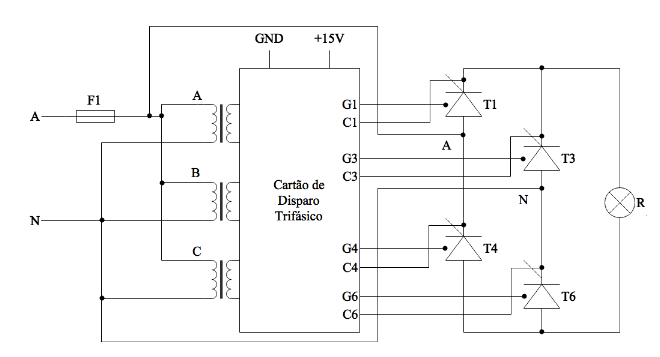
\includegraphics[width=\linewidth]{dados/resq}
	\caption{Diagrama para montagem do retificador monofásico de onda completa totalmente controlado}
	\label{fig:resq}
\end{figure}

Extraímos a curva de tensão na carga (figura \ref{fig:rvo}) e a tensão nos tiristores 3 (figura \ref{fig:rvt3}) e 6 (figura \ref{fig:rvt6}) para um ângulo de disparo $\alpha\ =\ 60^\circ$.
\begin{figure}[H]
	\centering
	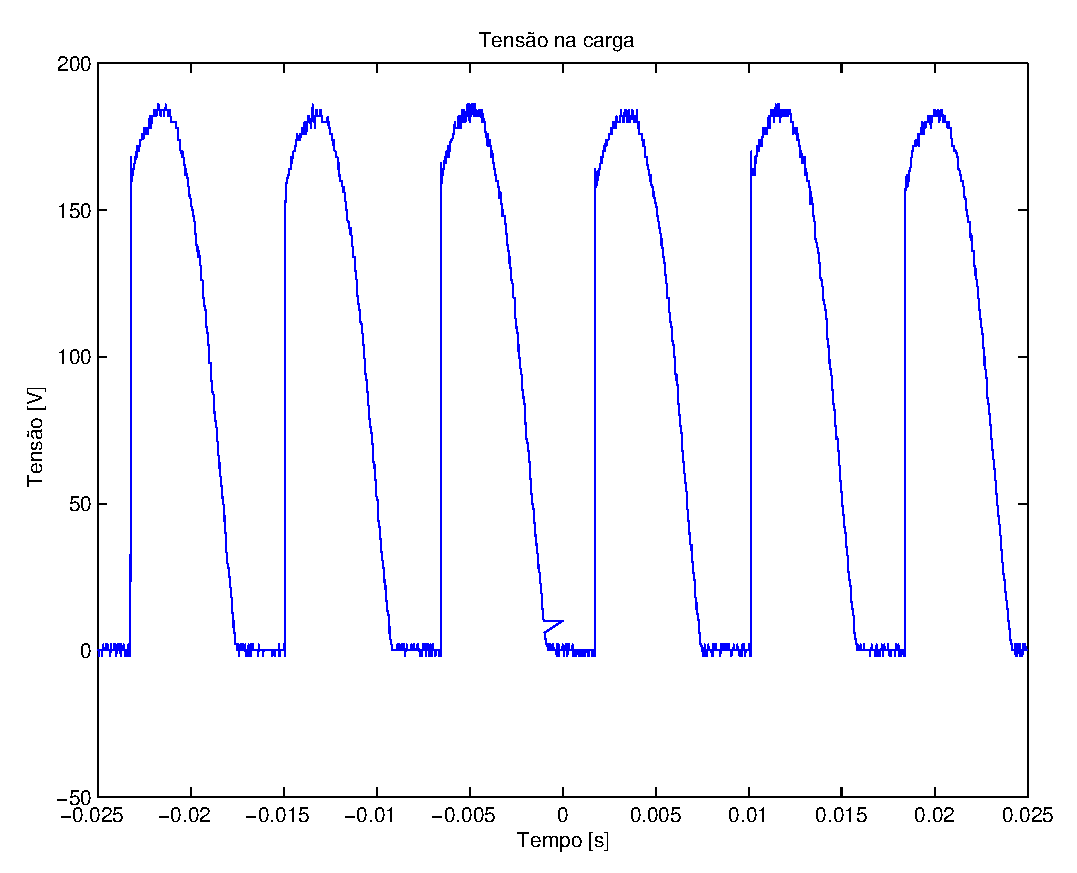
\includegraphics[width=0.7\linewidth]{matlab/r_vo}
	\caption{Tensão na carga para retificador monofásico com carga R}
	\label{fig:rvo}
\end{figure}
\begin{figure}[H]
	\centering
	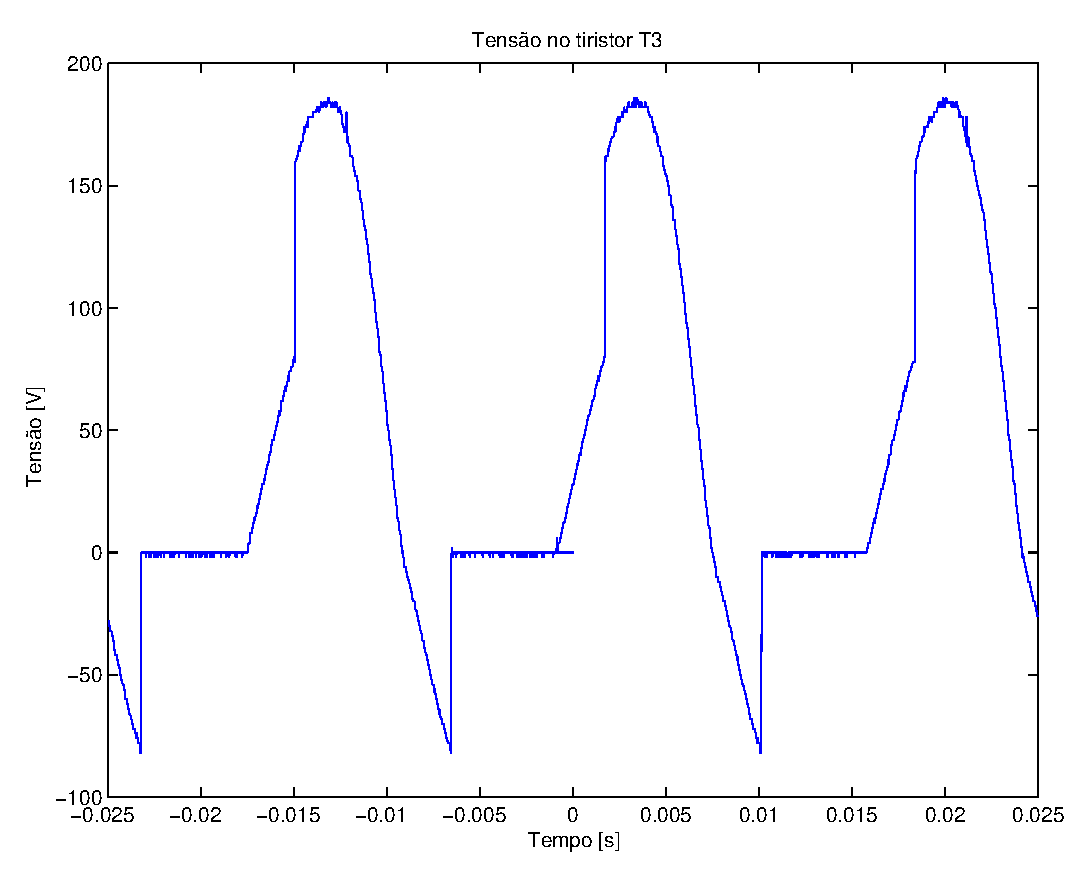
\includegraphics[width=0.7\linewidth]{matlab/r_vt3}
	\caption{Tensão no tiristor 3 para retificador monofásico com carga R}
	\label{fig:rvt3}
\end{figure}
\begin{figure}[H]
	\centering
	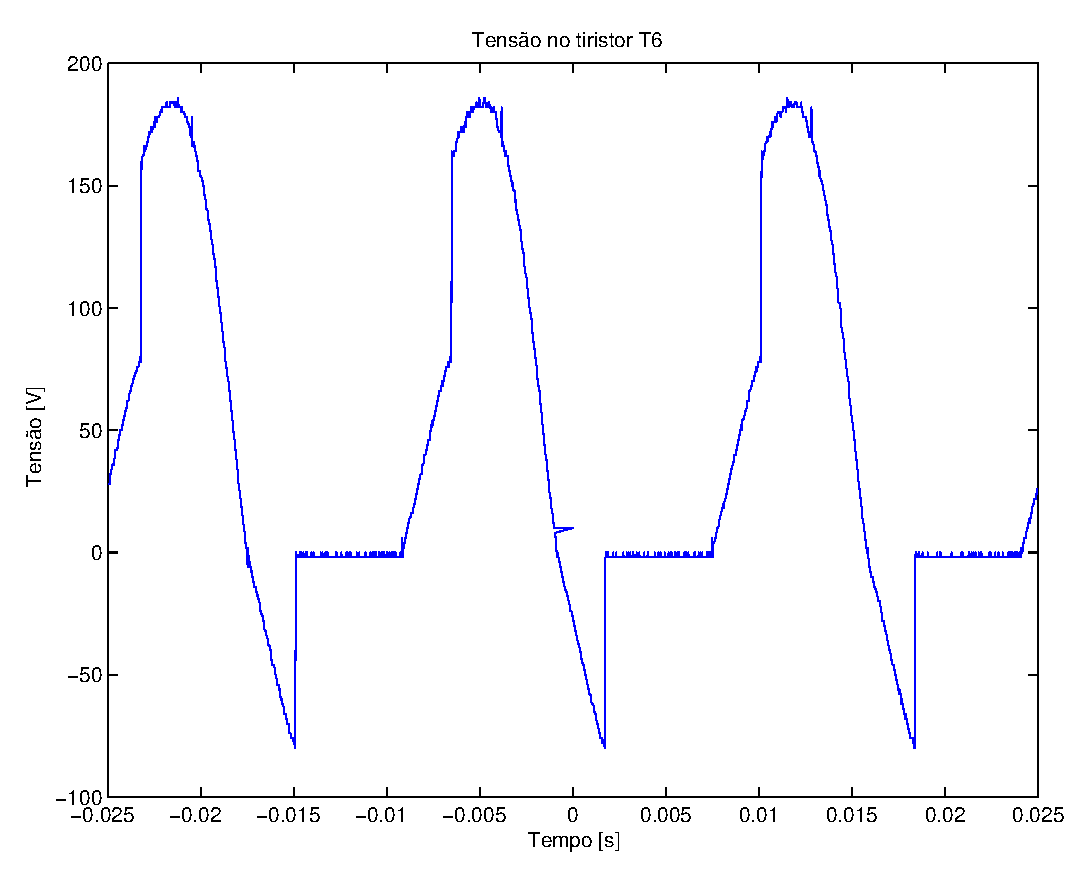
\includegraphics[width=0.7\linewidth]{matlab/r_vt6}
	\caption{Tensão no tiristor 6 para retificador monofásico com carga R}
	\label{fig:rvt6}
\end{figure}

Medimos a tensão média e efetiva na carga, obtendo os seguintes valores:
\begin{equation}
\overline{Vo} = 46.6080\ V
\end{equation}
\begin{equation}
Vo_{rms} =  62.2060\ V
\end{equation}

Podemos calcular a tensão média teórica sobre a carga através da equação \ref{eq:rmean}
\begin{equation}
	\overline{Vr} = \frac{1}{\pi} \int_{\alpha}^{\pi}{Vs sin(\theta)d\theta} = \frac{Vs (1 + cos(\alpha))}{\pi}
	\label{eq:rmean}
\end{equation}
Para calcular o valor efetivo da tensão sobre a carga utilizamos a equação \ref{eq:rrms}.
\begin{equation}
	Vr_{rms} = \sqrt{\frac{1}{\pi} \int_{\alpha}^{\pi}{(Vs sin(\theta))^2 d\theta}} = \frac{Vs \sqrt{\pi + \frac{sin(2\alpha)}{2}- \alpha }}{\sqrt{2 \pi}} 
	\label{eq:rrms}
\end{equation}
Varrendo o ângulo de disparo $\alpha$ entre $0^\circ$ e $180^\circ$ comparamos os valores teóricos e medidos para a tensão (figura \ref{fig:rvrr}) e corrente (figura \ref{fig:rirr}) sobre a carga
\begin{figure}[H]
	\centering
	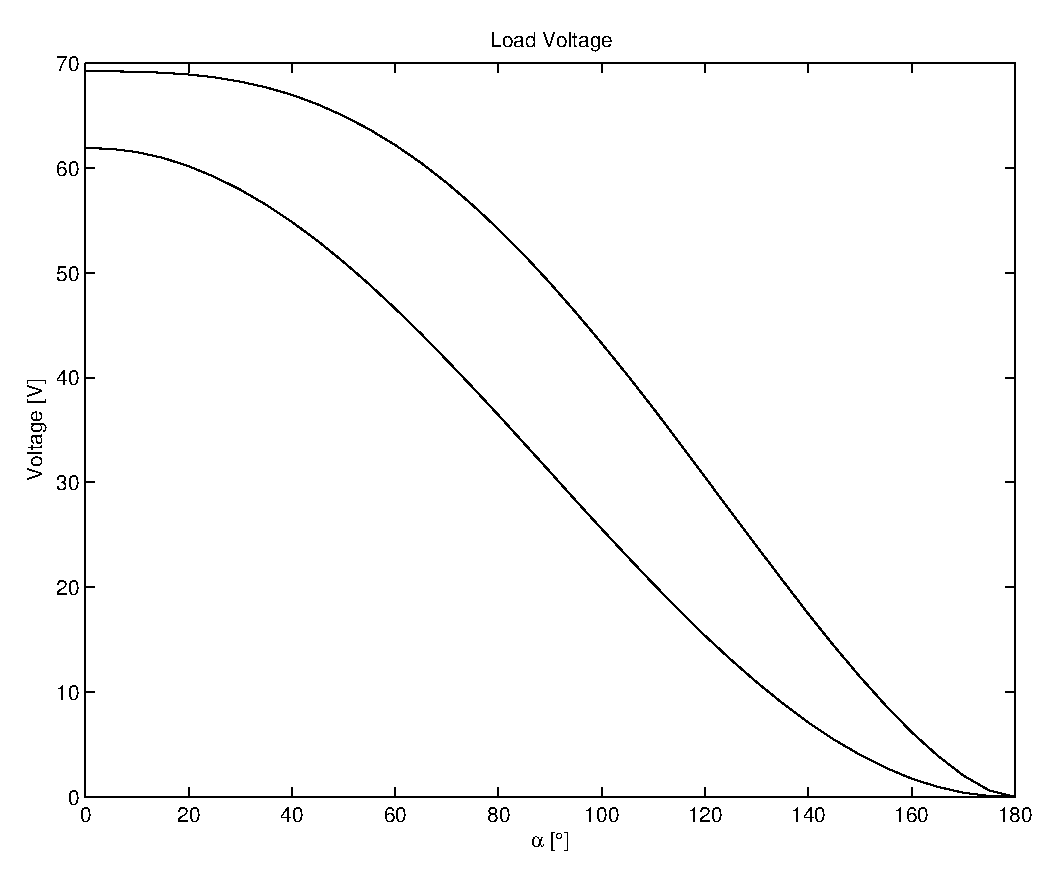
\includegraphics[width=0.7\linewidth]{matlab/r_vrr}
	\caption{Tensão na carga média e efetiva em função do ângulo de disparo}
	\label{fig:rvrr}
\end{figure}
\begin{figure}[H]
	\centering
	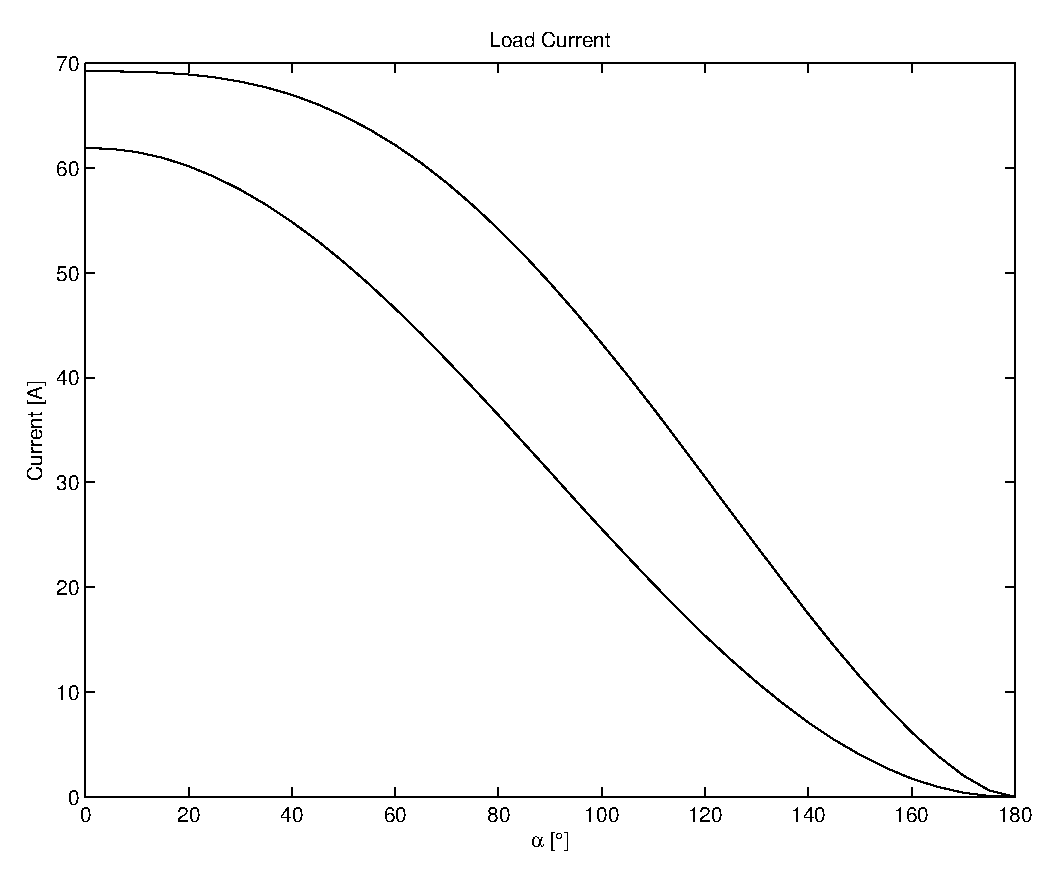
\includegraphics[width=0.7\linewidth]{matlab/r_irr}
	\caption{Corrente na carga média e efetiva em função do ângulo de disparo}
	\label{fig:rirr}
\end{figure}
Como podemos ver os valores obtidos são um pouco menores dos que os esperados teoricamente, isso se deve às imprecisões numéricas da simulação, à queda de tensão introduzida pelos diodos, ao pequeno período de amostragem, entre outros fatores.

Calculamos o fator de retificação para um ângulo de disparo $\alpha\ =\ 60^\circ$ usando a equação \ref{eq:rf}.
\begin{equation}
	\sigma = \frac{\overline{P}}{P_{rms}} = \frac{\overline{Vr}^2}{Vr_{rms}^2}
	\label{eq:rf}
\end{equation}

\begin{equation}
	\sigma = 0.5614
\end{equation}

Encontramos por fim o fator de forma para um ângulo de disparo $\alpha\ =\ 60^\circ$ usando a equação \ref{eq:ff}.
\begin{equation}
FF = \frac{\overline{Vr}}{Vr_{rms}}
\label{eq:ff}
\end{equation}

\begin{equation}
FF = 1.3347
\end{equation}


\section{Carga RL}
Conectamos então um indutor em série com o resistor conforme mostrado na figura \ref{fig:rlsim}.
\begin{figure}[H]
	\centering
	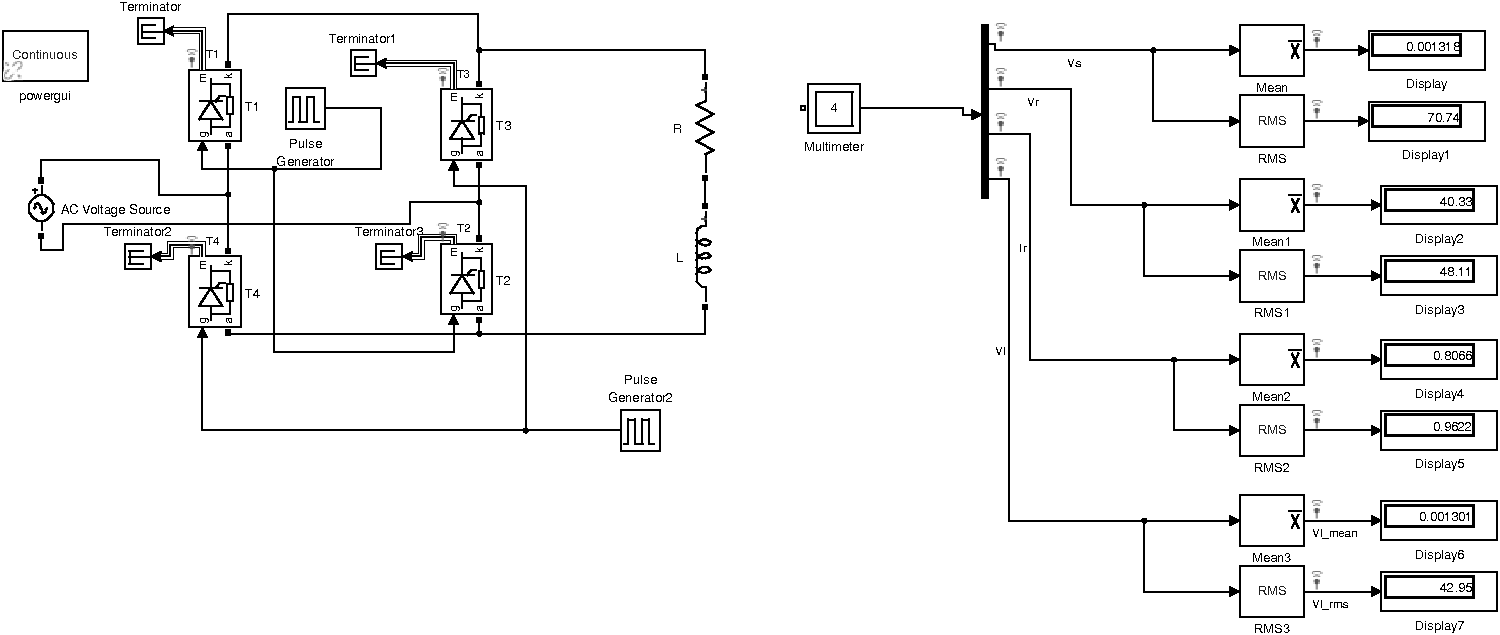
\includegraphics[width=\linewidth]{matlab/rlsim}
	\caption{Esquema para simulação do retificador monofásico controlado com carga RL}
	\label{fig:rlsim}
\end{figure}

Simulamos o circuito para uma indutância $L\ =\ 100mH$ e um ângulo de disparo $\alpha\ =\ 60^\circ$. Extraímos dessa simulação as curvas de tensão (figura \ref{fig:rlvr}) e corrente (figura \ref{fig:rlir}) no resistor e de tensão no indutor (figura \ref{fig:rlvl}) para dois períodos da fonte.
\begin{figure}[H]
	\centering
	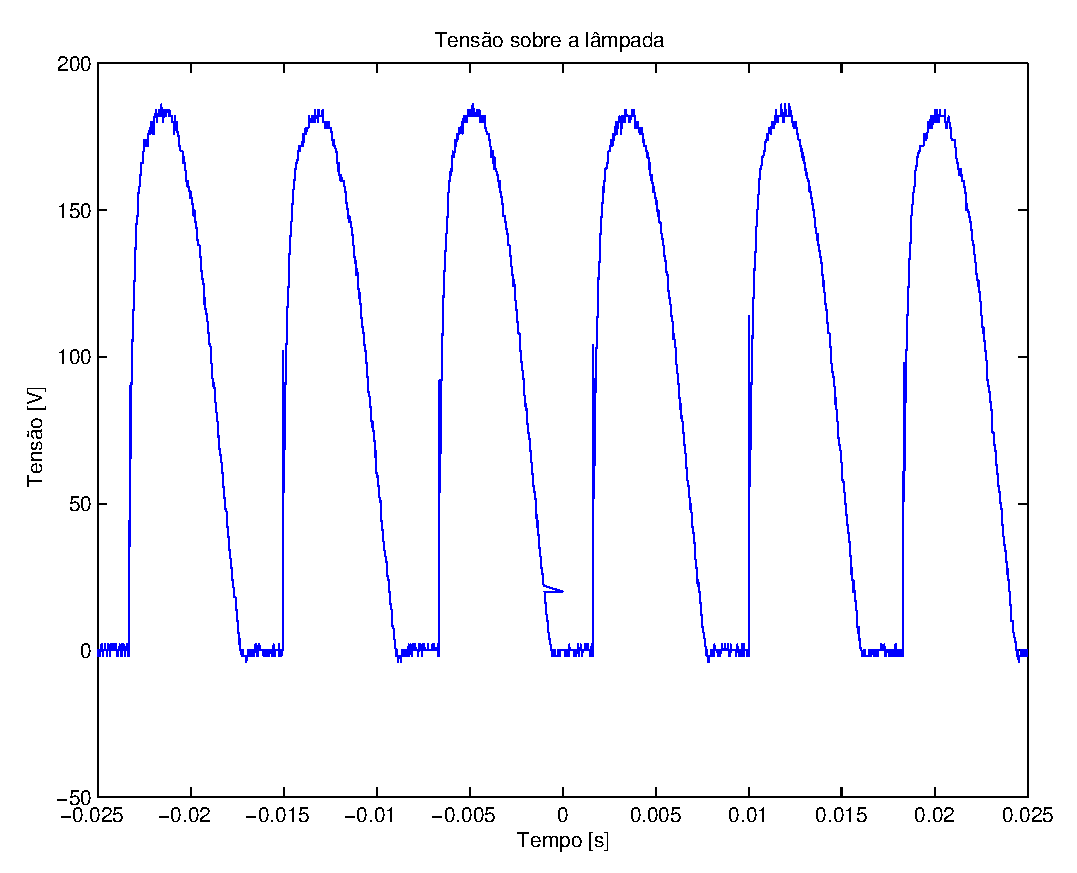
\includegraphics[width=0.7\linewidth]{matlab/rl_vr}
	\caption{Tensão no resistor para retificador monofásico com carga RL (100mH)}
	\label{fig:rlvr}
\end{figure}
\begin{figure}[H]
	\centering
	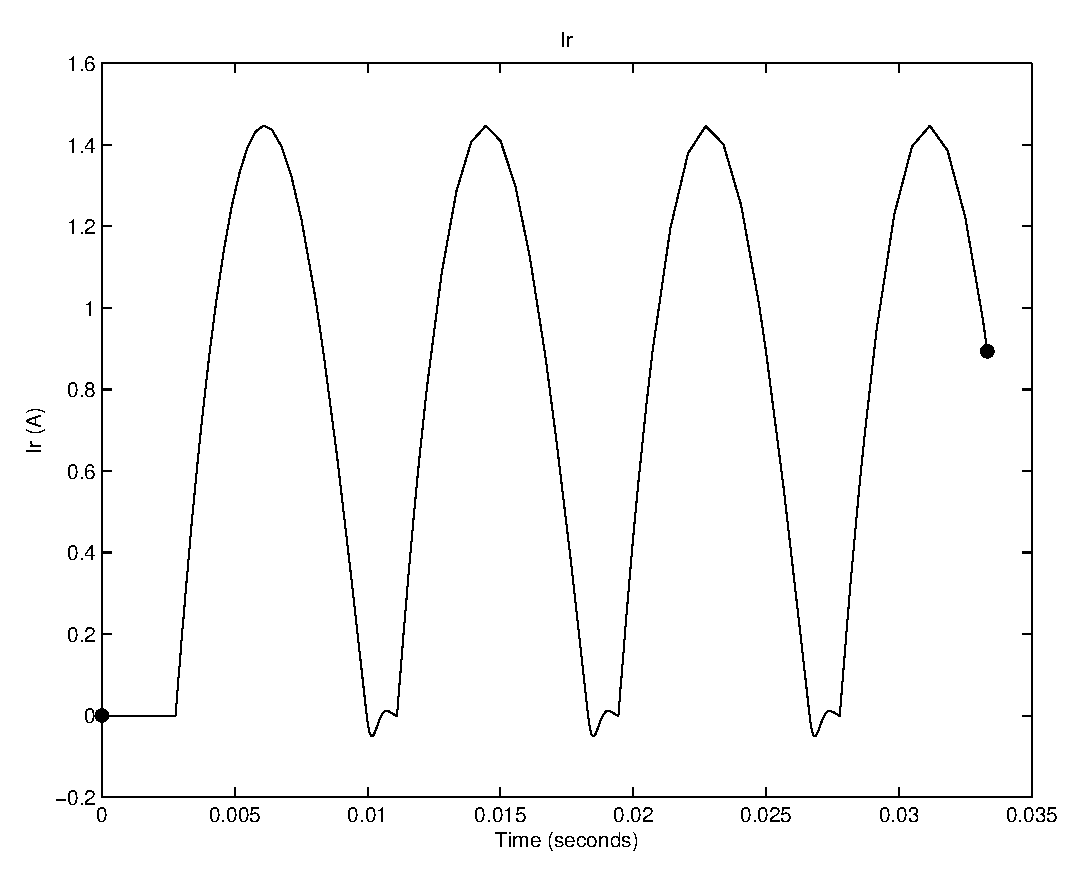
\includegraphics[width=0.7\linewidth]{matlab/rl_ir}
	\caption{Corrente no resistor para retificador monofásico com carga RL (100mH)}
	\label{fig:rlir}
\end{figure}
\begin{figure}[H]
	\centering
	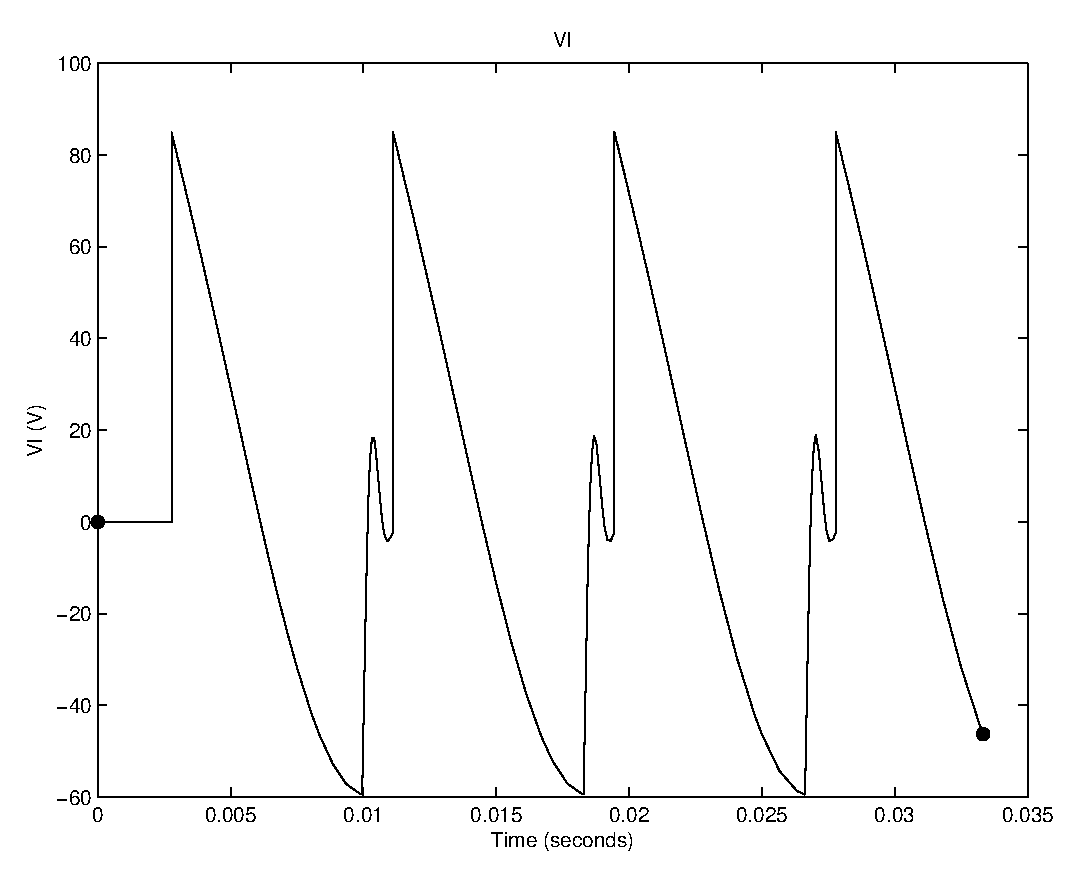
\includegraphics[width=0.7\linewidth]{matlab/rl_vl}
	\caption{Tensão no indutor para retificador monofásico com carga RL (100mH)}
	\label{fig:rlvl}
\end{figure}
Medimos as tensões e correntes médias e efetivas na resistência R, obtendo os seguintes valores:
\begin{equation}
\overline{Vr} = 40.3318\ V
\end{equation}
\begin{equation}
\overline{Ir} =  0.8066\ A
\end{equation}
\begin{equation}
Vr_{rms} =  48.1121\ V
\end{equation}
\begin{equation}
Ir_{rms} =   0.9622\ A
\end{equation}

Calculamos o fator de retificação usando a equação \ref{eq:rf}.
\begin{equation}
\sigma = 0.7027
\end{equation}

Encontramos também o fator de forma usando a equação \ref{eq:ff}.
\begin{equation}
FF = 1.1929
\end{equation}

Simulamos então circuito com uma indutância $L\ =\ 1H$ e um ângulo de disparo $\alpha\ =\ 60^\circ$. Extraímos dessa simulação as curvas de tensão (figura \ref{fig:rl2vr}) e corrente (figura \ref{fig:rl2ir}) no resistor e de tensão no indutor (figura \ref{fig:rl2vl}) para quinze períodos da fonte.
\begin{figure}[H]
	\centering
	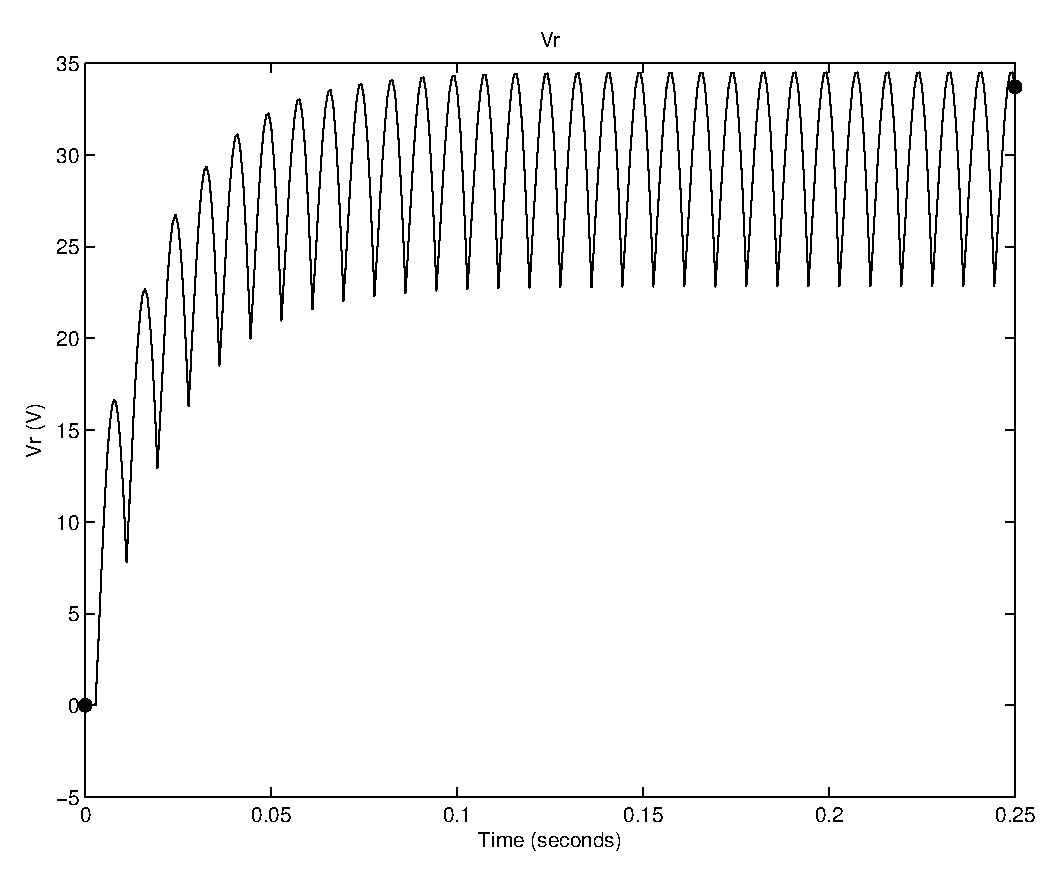
\includegraphics[width=0.7\linewidth]{matlab/rl2_vr}
	\caption{Tensão no resistor para retificador monofásico com carga RL (1H)}
	\label{fig:rl2vr}
\end{figure}
\begin{figure}[H]
	\centering
	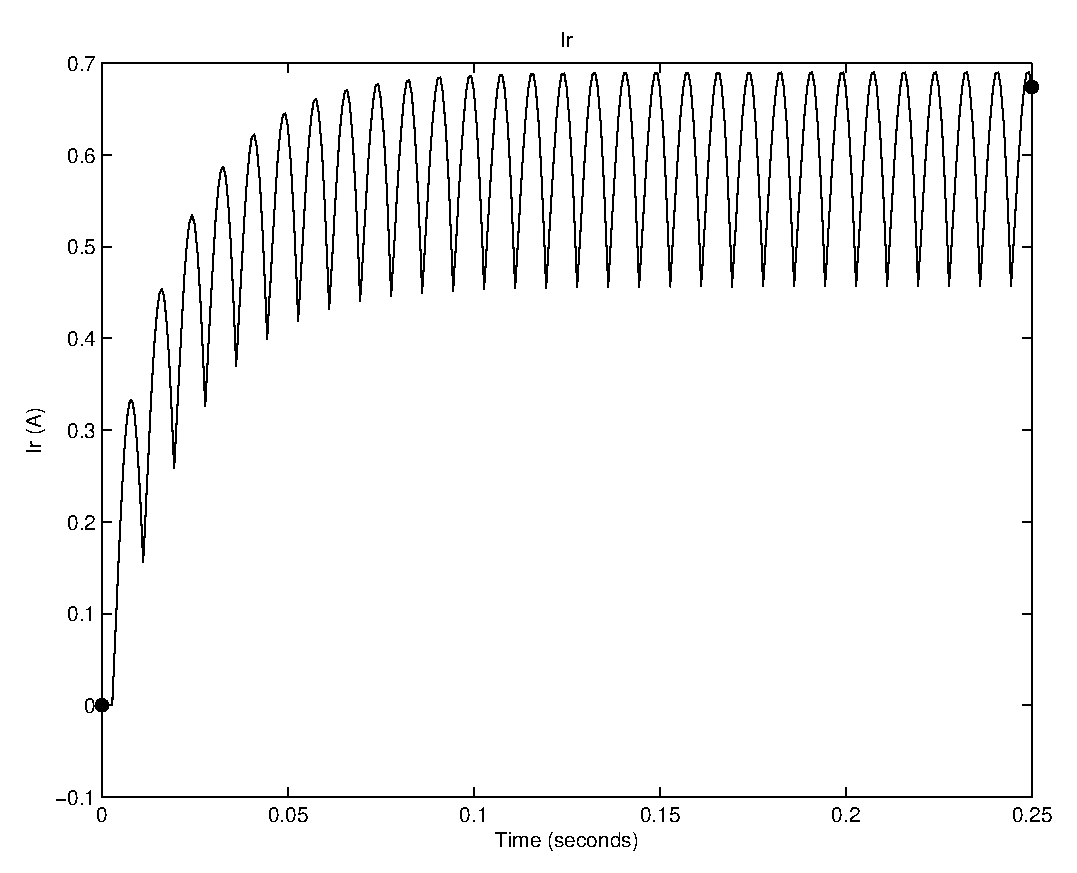
\includegraphics[width=0.7\linewidth]{matlab/rl2_ir}
	\caption{Corrente no resistor para retificador monofásico com carga RL (1H)}
	\label{fig:rl2ir}
\end{figure}
\begin{figure}[H]
	\centering
	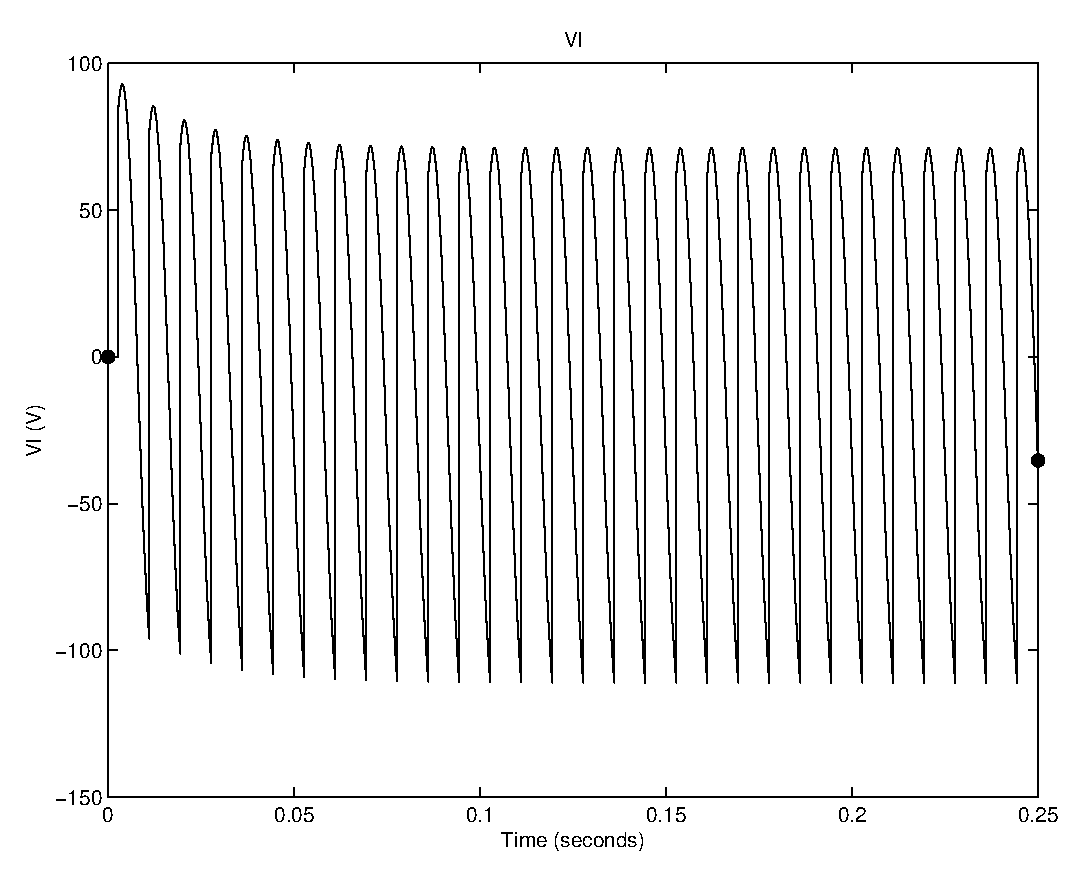
\includegraphics[width=0.7\linewidth]{matlab/rl2_vl}
	\caption{Tensão no indutor para retificador monofásico com carga RL (1H)}
	\label{fig:rl2vl}
\end{figure}
Medimos as tensões e correntes médias e efetivas na resistência R, obtendo os seguintes valores:
\begin{equation}
\overline{Vr} = 30.1911\ V
\end{equation}
\begin{equation}
\overline{Ir} =  0.6038\ A
\end{equation}
\begin{equation}
Vr_{rms} =  30.4340\ V
\end{equation}
\begin{equation}
Ir_{rms} =    0.6087\ A
\end{equation}
Sendo $\beta$ a defasagem introduzida pela carga indutiva:
\begin{equation}
	\beta = \arctan{(\frac{L\omega}{R})}
\end{equation}
Podemos calcular a tensão média teórica sobre a carga através da equação \ref{eq:rlmean}
\begin{equation}
\overline{Vr} = \frac{1}{\pi} \int_{\alpha}^{\pi + min(\alpha, \beta)}{Vs \sin{(\theta)}d\theta} = \frac{Vs (-\cos{(\pi + min(\alpha, \beta))} + \cos{(\alpha}))}{\pi}
\label{eq:rlmean}
\end{equation}
Para calcular o valor efetivo da tensão sobre a carga utilizamos a equação \ref{eq:rlrms}.
\begin{equation}
Vr_{rms} = \sqrt{\frac{1}{\pi} \int_{\alpha}^{\pi + min(\alpha, \beta)}{(Vs \sin(\theta))^2 d\theta}} = \frac{Vs \sqrt{\pi + min(\alpha, \beta) + \frac{sin(2\alpha)}{2} - \frac{sin(2(\pi + min(\alpha, \beta)))}{2} - \alpha }}{\sqrt{2 \pi}} 
\label{eq:rlrms}
\end{equation}

Calculamos o fator de retificação usando a equação \ref{eq:rf}.
\begin{equation}
\sigma =  0.9841
\end{equation}

Encontramos também o fator de forma usando a equação \ref{eq:ff}.
\begin{equation}
FF = 1.0080
\end{equation}

Podemos ver que ao introduzir uma carga indutiva os tiristores continuam conduzindo mesmo que a tensão sobre eles seja negativa (contanto que a corrente continue positiva). Isso causa uma redução da tensão média na carga. Ao mesmo tempo, o indutor, uma vez carregado evita variações bruscas na corrente sobre a carga (possivelmente evitando que ela chegue a zero), aumentando o alisamento (e consequentemente melhorando o fator de forma e o de retificação) de maneira proporcional ao valor da indutância.

Para os dois valores de indutância nós medimos uma tensão média praticamente nula no indutor. Esse resultado é esperado uma vez que:
\begin{equation}
	\overline{Vl} = \frac{1}{T}\int_{0}^{T}Vl dt = \frac{1}{T}\int_{0}^{T}\frac{LdI}{dt} dt = \frac{LI}{T}\bigg\rvert_0^T
\end{equation}
Como nossa resposta é periódica, sabemos que $I(0)\ =\ I(T)$ logo:
\begin{equation}
	\overline{Vl} = 0
\end{equation}

\section{Carga RC}
Conectamos então um capacitor em paralelo com o resistor conforme mostrado na figura \ref{fig:rcsim}.
\begin{figure}[H]
	\centering
	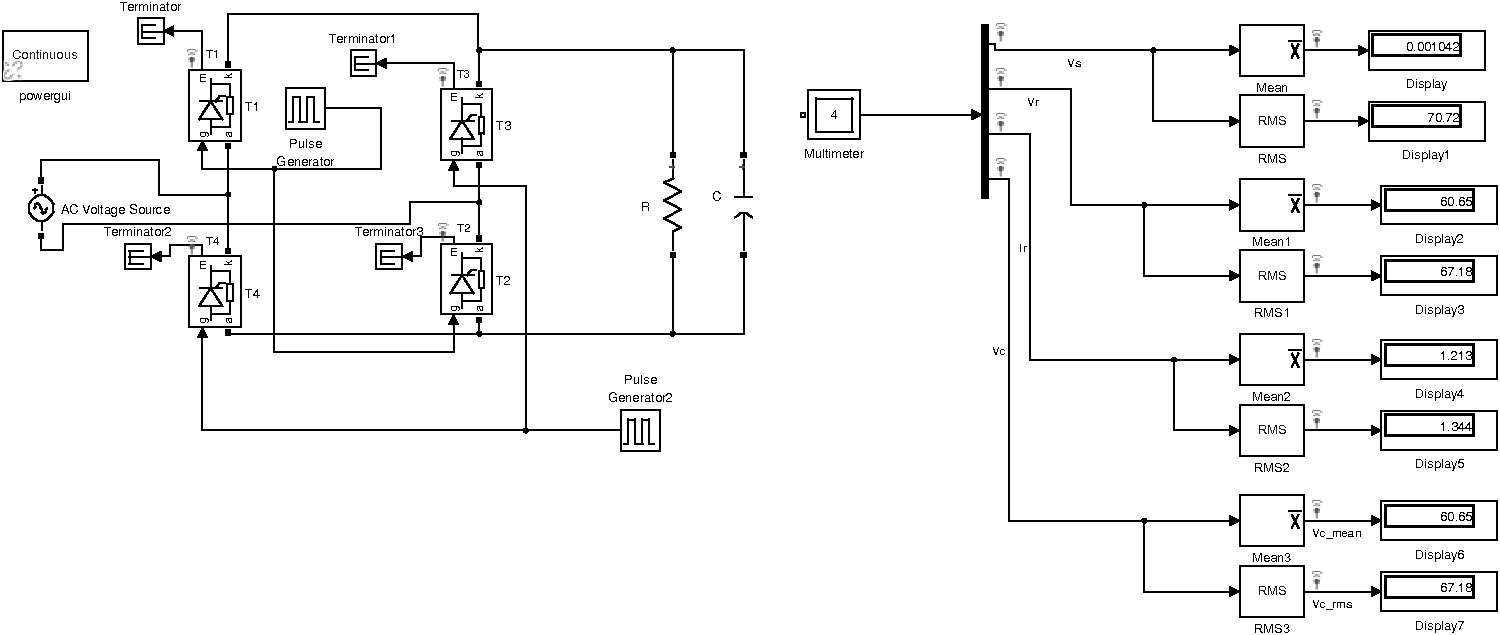
\includegraphics[width=\linewidth]{matlab/rcsim}
	\caption{Esquema para simulação do retificador monofásico controlado com carga RC}
	\label{fig:rcsim}
\end{figure}

Simulamos o circuito para uma capacitância $C\ =\ 100\mu F$ e um ângulo de disparo $\alpha\ =\ 60^\circ$. Extraímos dessa simulação as curvas de tensão (figura \ref{fig:rcvr}) e corrente (figura \ref{fig:rcir}) no resistor para dois períodos da fonte.
\begin{figure}[H]
	\centering
	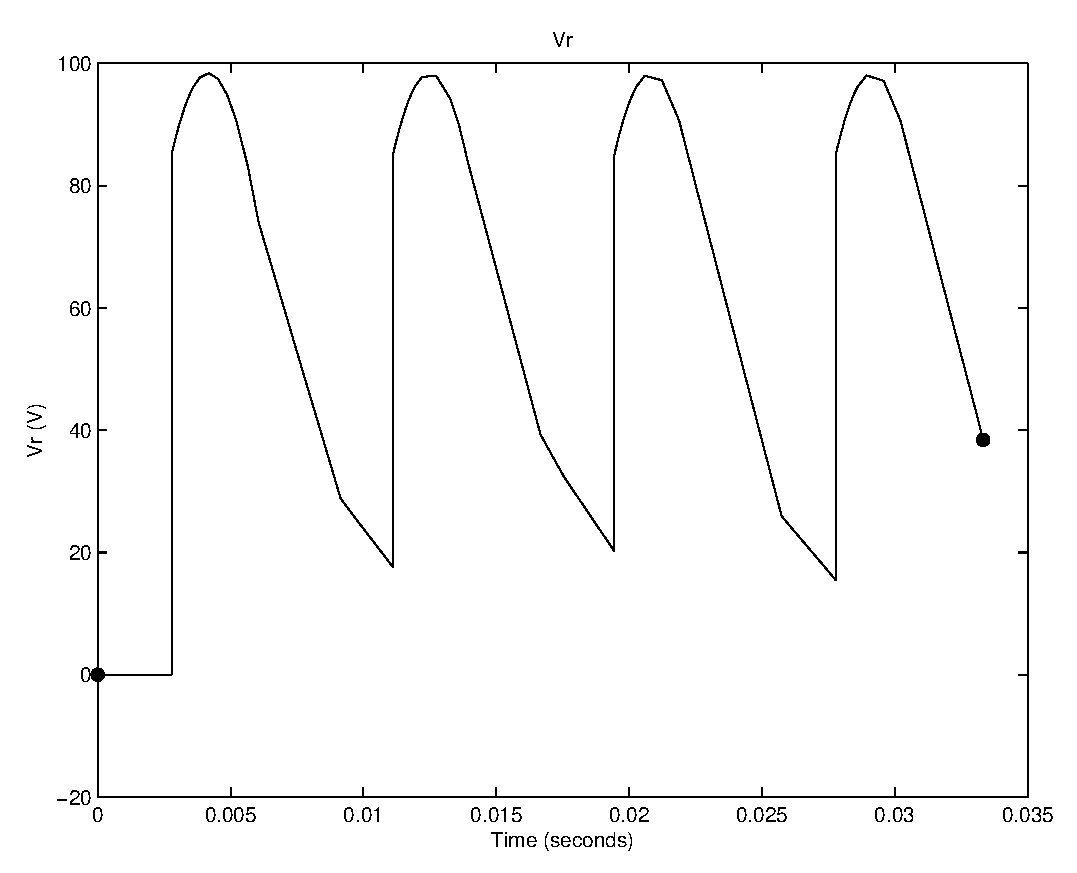
\includegraphics[width=0.7\linewidth]{matlab/rc_vr}
	\caption{Tensão no resistor para retificador monofásico com carga RC ($100\mu F$)}
	\label{fig:rcvr}
\end{figure}
\begin{figure}[H]
	\centering
	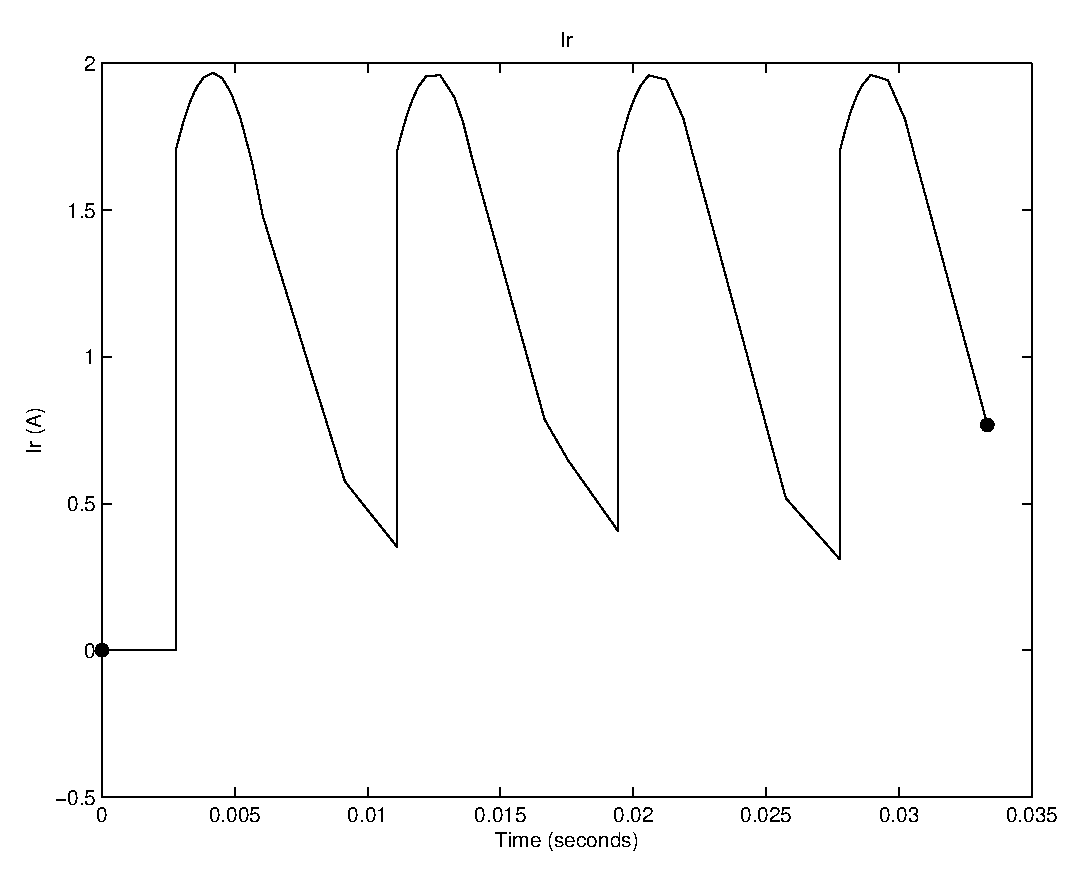
\includegraphics[width=0.7\linewidth]{matlab/rc_ir}
	\caption{Corrente no resistor para retificador monofásico com carga RC ($100\mu F$)}
	\label{fig:rcir}
\end{figure}

Medimos as tensões e correntes médias e efetivas na resistência R, obtendo os seguintes valores:
\begin{equation}
\overline{Vr} = 60.6456\ V
\end{equation}
\begin{equation}
\overline{Ir} = 1.2129\ A
\end{equation}
\begin{equation}
Vr_{rms} = 67.1804\ V
\end{equation}
\begin{equation}
Ir_{rms} = 1.3436\ A
\end{equation}

Calculamos o fator de retificação usando a equação \ref{eq:rf}.
\begin{equation}
\sigma = 0.8149
\end{equation}

Encontramos também o fator de forma usando a equação \ref{eq:ff}.
\begin{equation}
FF = 1.1078
\end{equation}

Simulamos então circuito com uma capacitância $C\ =\ 1mF$ e um ângulo de disparo $\alpha\ =\ 60^\circ$. Extraímos dessa simulação as curvas de tensão (figura \ref{fig:rc2vr}) e corrente (figura \ref{fig:rc2ir}) no resistor para dois períodos da fonte.
\begin{figure}[H]
	\centering
	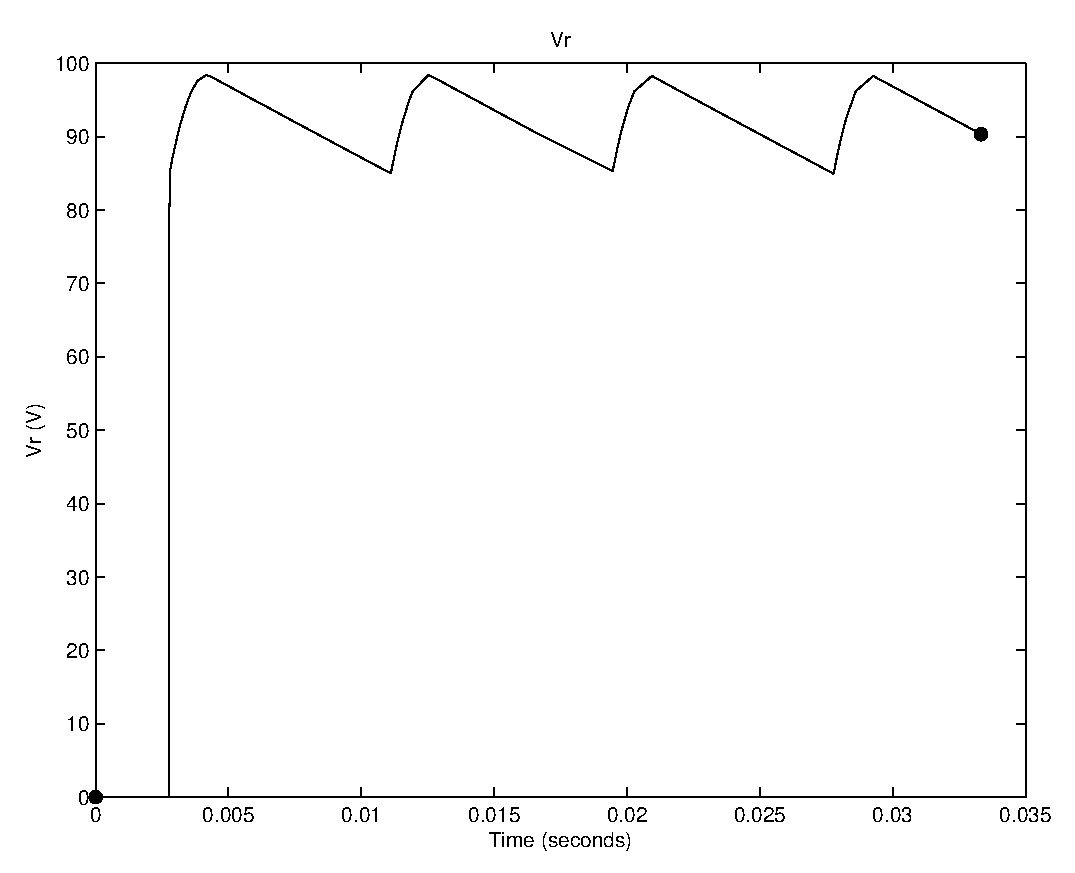
\includegraphics[width=0.7\linewidth]{matlab/rc2_vr}
	\caption{Tensão no resistor para retificador monofásico com carga RC ($1mF$)}
	\label{fig:rc2vr}
\end{figure}
\begin{figure}[H]
	\centering
	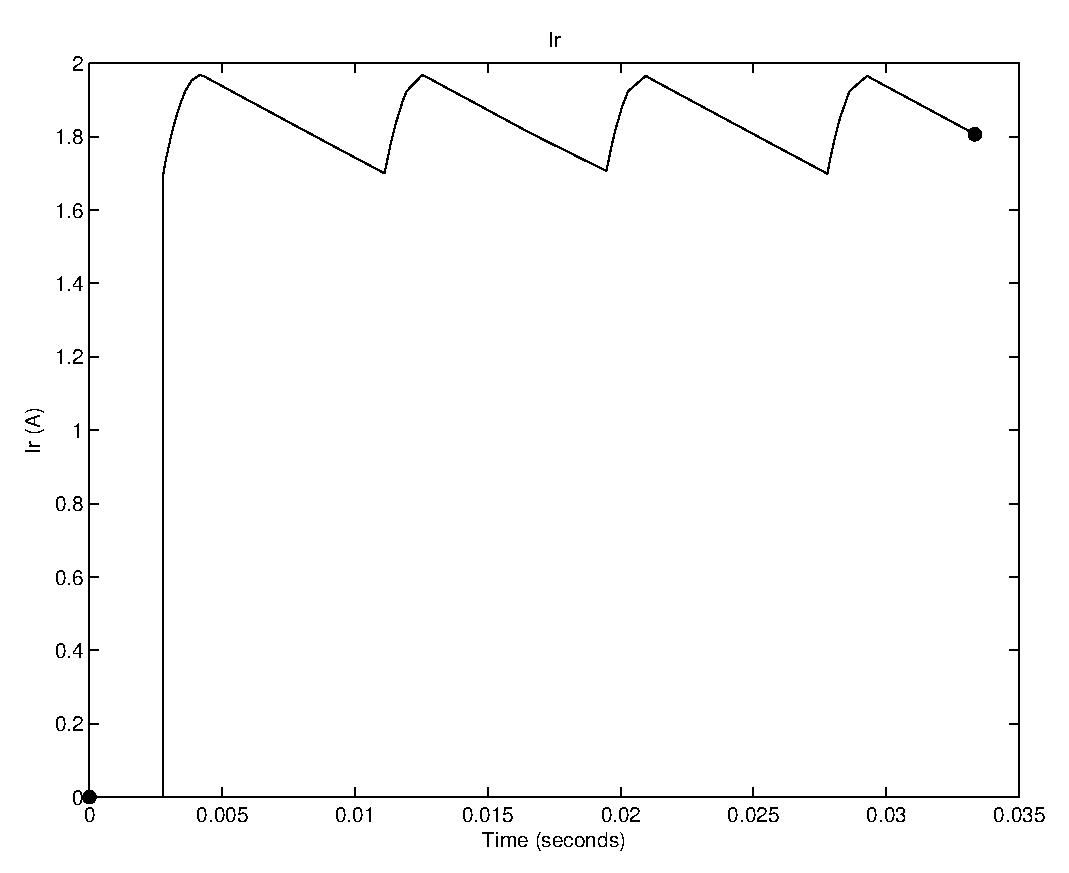
\includegraphics[width=0.7\linewidth]{matlab/rc2_ir}
	\caption{Corrente no resistor para retificador monofásico com carga RC ($1mF$)}
	\label{fig:rc2ir}
\end{figure}
Medimos as tensões e correntes médias e efetivas na resistência R, obtendo os seguintes valores:
\begin{equation}
\overline{Vr} = 92.0838\ V
\end{equation}
\begin{equation}
\overline{Ir} = 1.8417\ A
\end{equation}
\begin{equation}
Vr_{rms} = 92.1690\ V
\end{equation}
\begin{equation}
Ir_{rms} = 1.8434\ A
\end{equation}

Calculamos o fator de retificação usando a equação \ref{eq:rf}.
\begin{equation}
\sigma = 0.9982
\end{equation}

Encontramos também o fator de forma usando a equação \ref{eq:ff}.
\begin{equation}
FF = 1.0009
\end{equation}

Ao introduzir uma carga capacitiva esta armazenará energia, liberando-a quando a tensão sobre o resistor diminuí. Essa energia liberada causa uma retificação da tensão sobre o resistor, de maneira proporcional à capacitância, obtendo uma curva de tensão quase linear com ótimos fatores de forma e de retificação.

\bibliography{mybib}
\end{document}

